% --
% adversarial

\section{Adversarial Pre-Training}\label{sec:nn_adv}
In adversarial neural network training, two separate neural networks are competing against each other in an adversary task.
This competition of the two networks motivates them to improve their performance and beat the other network.
The application of GANs, as already explained in \rsec{prev_nn_adv} and \rsec{nn_theory_gan}, is an interesting subject in research and the questions whether the obtained weights from the training of the Generator (G) and Discriminator (D) network can contribute to better the performances in equivalent models, arises.
In the following, the training algorithms are explained in more detail, such as the loss functions used for G and D.
The transfer of weights can be done for training instances on small subsets of labels or the whole network by regarding all labels at once in a single training instance.
The transferring technique of training instances on small subsets of labels is denoted as \emph{adversarial label train} and the transfer of weights from a whole network with all labels is named as \emph{adversarial dual train}.
Only the adversarial label train is explained in detail because the adversarial dual train is straight forward once the adversarial label train is understood.
Note that the adversarial pre-training performs only on the \texttt{adv-d-jim} and \texttt{adv-g-jim} models to update the \texttt{conv-jim} model.
Those models were already described in \rsec{nn_arch}.


% --
% training GANs

\subsection{Training Generative Adversarial Neural Networks}\label{sec:nn_adv_train}
The interesting part in training GANs is how the Generator and Discriminator models are updated in each training step and which loss functions were used.
In \req{nn_theory_gan} the game is notated as min-max game, from which the loss of D, denoted as $l_D$, can be described for one specific training example $i$ of a batch as:
\begin{equation}
  l_D(x_i, z_i, G) = l(D(x_i), y_r) + l(D(G(z_i)), y_f)
\end{equation}
where $l$ is the binary cross-entropy loss described in \req{nn_theory_binary_cross_entropy}, $D: \mathcal{X} \mapsto [0, 1]$ and $G: \mathcal{Z} \mapsto \mathcal{X}$ are the Discriminator and Generator model, $x_i \in \mathcal{X}$ is a data example, $z_i \in \mathcal{Z}$ is a randomly sampled latent variable, $y_r = 1$ is the real label and $y_f = 0$ the fake label for that specific example $i$.
In contrast the loss of the Generators, denoted as $l_G$, is given by:
\begin{equation}
  l_G(z_i, D) =  l(D(G(z_i)), y_r)
\end{equation}
with $y_r$ as real label to perform maximization of $\log D(G(\bm{z}))$ as described in \rsec{nn_theory_gan}.

An extended approach, so that G produces samples specifically similar to the data distribution and does not drift off into creating unrealistic fakes of noisy samples to fake D, is to incorporate a similarity term with the \emph{cosine similarity} defined by:
\begin{equation}
  s(\bm{x_1}, \bm{x_2}) = \frac{\bm{x_1}^T \bm{x_2}}{\norm{\bm{x_1}}_2 \cdot \norm{\bm{x_2}}_2 + \epsilon} 
\end{equation}
where $s : (\mathcal{X}, \mathcal{X}) \mapsto [0, 1]$ is the cosine similarity function, $\bm{x_1}$ and $\bm{x_2}$ are two vectors for similarity measure and $\epsilon$ is a small number, such that no division by zero is possible.
With the similarity loss incorporated, $l_G$ gets:
\begin{equation}
  l_G(x_i, z_i, D) =  l(D(G(z_i)), y_r) + \lambda \left(1 - \frac{1}{C} \sum_{c=0}^{C} s(\hat{\bm{e}}_c^T x_i , \hat{\bm{e}}_c^T G(z_i)) \right)
\end{equation}
where $\hat{\bm{e}}_c \in \{1, 0\}^C$ is a unit vector representing one cepstral coefficient of the Mel Frequency Cepstral Coefficient (MFCC) data $x_i \in \mathcal{X} = \R^{C \times M}$ with a total number of $C$ MFCC coefficients and $M$ frames.
Further $\lambda$ is a trade-off factor between data similarity and fake loss from D.
For the experiments in \rsec{exp_adv}, $\lambda = 5$ was chosen.

The update of D and G performs in each training step by backpropagating the obtained losses.
However it is more appealing to update D for a certain numbers of training steps with no update of G and then alternating to updates of G without updating D.
This will give either D or G some update steps to improve in their specific adversarial task of either discriminating or generating.
In this thesis the training steps for updating either D or G were selected to 2 epochs.
Note that an epoch consists of several training steps depending on the batch size and amount of data.
This can vary for the experiments, however it does not dramatically influence the overall end results.


% --
% label train

\subsection{Adversarial Label Train}
Adversarial label train is the transfer of weights of convolutional filters (kernels) trained on multiple GAN training instances on subsets of all labels.
For instance if the label set in the class dictionary is \{\enquote{left}, \enquote{right}\} then a separate training instance may focus on the label \enquote{left} and another on the label \enquote{right}.
It is important to assign a specific number of filters to each label train instance.
For example, each label train gets 8 filters in the first convolutional layer.
\rfig{nn_adv_label_scheme} illustrates the label train scheme through 6 label train instances, such as used for the experiments in \rsec{exp_adv}.
\begin{figure}[!ht]
  \centering
    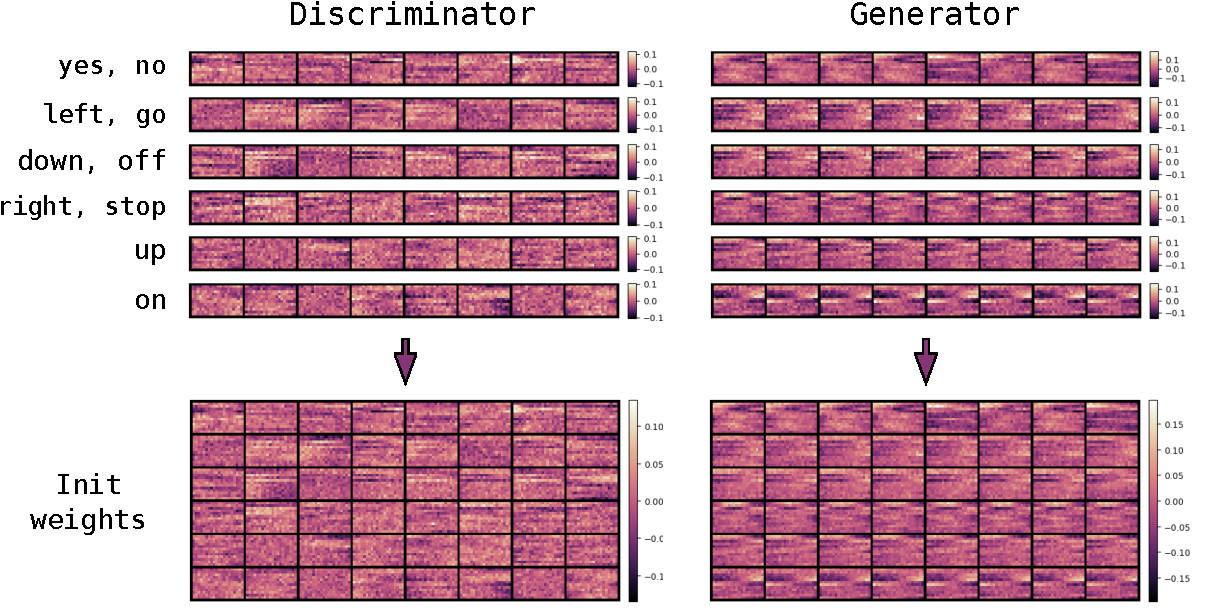
\includegraphics[width=0.85\textwidth]{./4_nn/figs/nn_adv_label_scheme.pdf}
  \caption{Label train scheme showing the first convolutional layers of \texttt{adv-d-jim}, \texttt{adv-g-jim} and \texttt{conv-jim} with 6 label subset as separate training instances using 100 epochs.}
  \label{fig:nn_adv_label_scheme}
\end{figure}
\FloatBarrier
\noindent
To further investigate the adversarial label train, the training results of the models \texttt{adv-d-jim}, \texttt{adv-g-jim} and \texttt{conv-jim} is provided in the following.
\rfig{nn_adv_loss_label} shows the training loss of an actual GAN training for the label subset \{\enquote{left}, \enquote{go}\}.
\begin{figure}[!ht]
  \centering
  \subfigure[100 epochs]{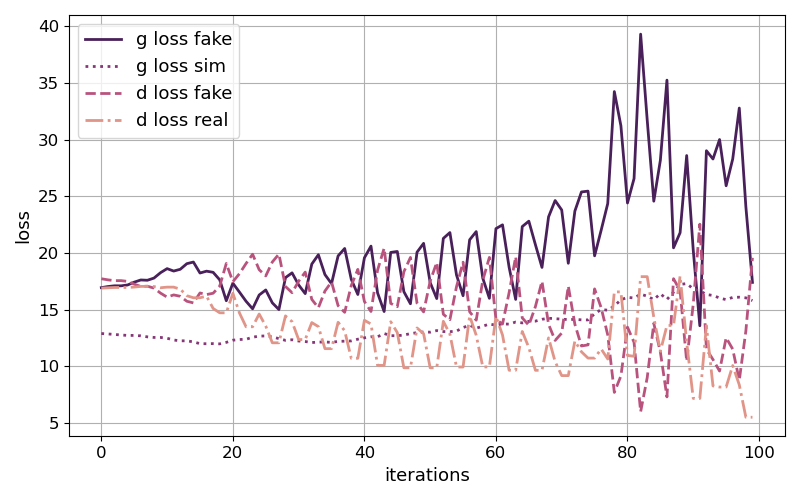
\includegraphics[width=0.45\textwidth]{./4_nn/figs/nn_adv_loss_label_it-100.png}}
  \subfigure[1000 epochs]{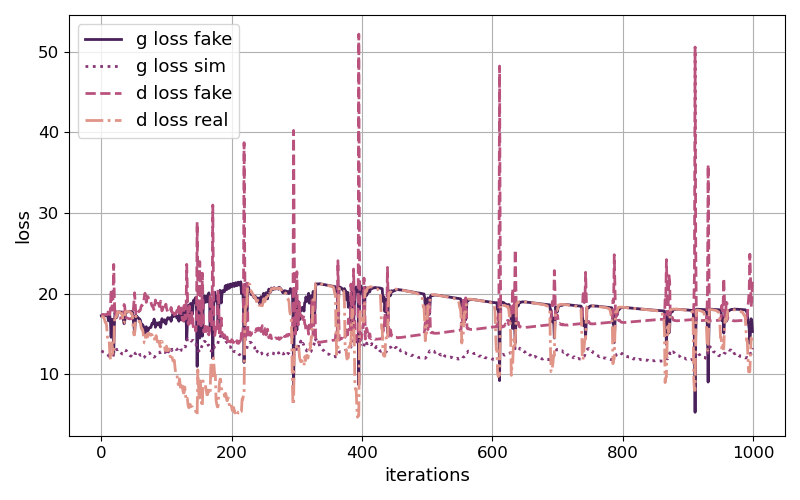
\includegraphics[width=0.45\textwidth]{./4_nn/figs/nn_adv_loss_label_it-1000.png}}
  \caption{Adversarial training loss of the label subset \{\enquote{left}, \enquote{go}\}.}
  \label{fig:nn_adv_loss_label}
\end{figure}
\FloatBarrier
\noindent
Note that the update of either the Discriminator or Generator model performs alternately every 2 training epochs, as described in \rsec{nn_adv_train}.
\rfig{nn_adv_fakes_label} shows the generation of fake images from G with different amounts of training epochs.
\begin{figure}[!ht]
  \centering
  \subfigure[100 epochs]{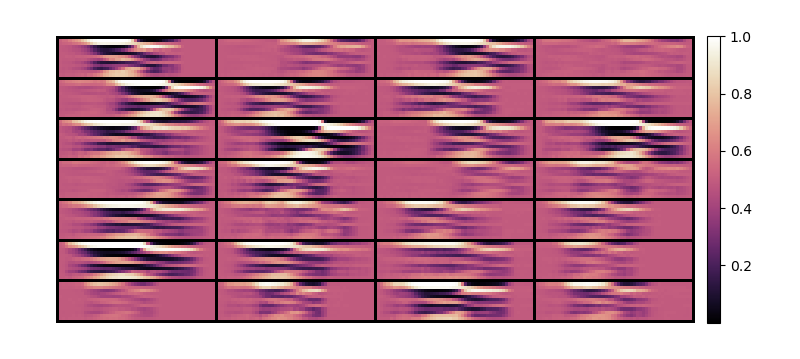
\includegraphics[width=0.45\textwidth]{./4_nn/figs/nn_adv_fakes_label_it-100.png}}
  \subfigure[1000 epochs]{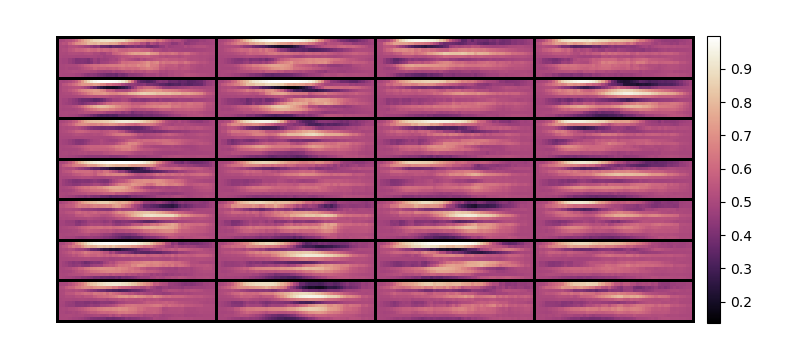
\includegraphics[width=0.45\textwidth]{./4_nn/figs/nn_adv_fakes_label_it-1000.png}}
  \caption{Generation of fake images of the label subset \{\enquote{left}, \enquote{go}\} with different amounts of epochs.}
  \label{fig:nn_adv_fakes_label}
\end{figure}
\FloatBarrier
\noindent
\rfig{nn_adv_label_weights_d} and \rfig{nn_adv_label_weights_g} show trained weights of the filters in the first convolutional layer of D and G respectively, obtained from an adversarial label train with different amount of epochs.
\begin{figure}[!ht]
  \centering
  \subfigure[D with 100 epochs]{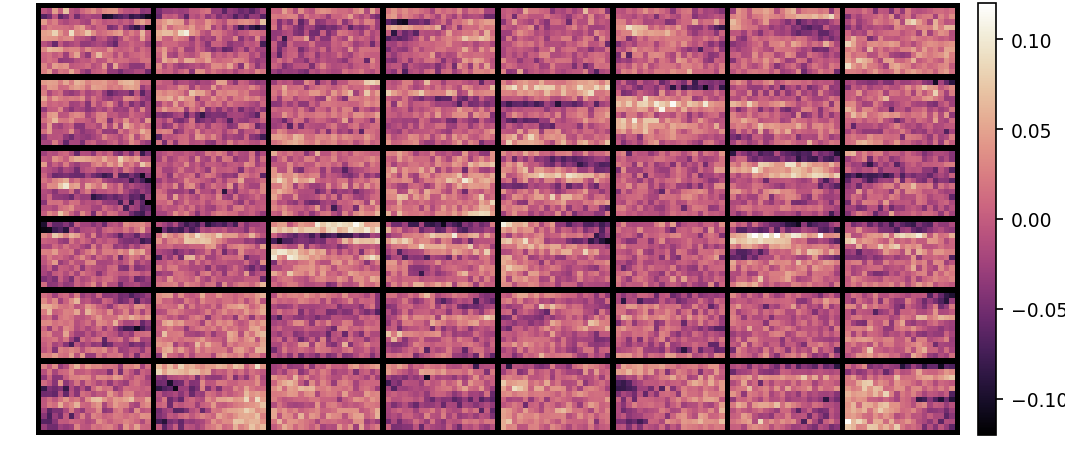
\includegraphics[width=0.45\textwidth]{./4_nn/figs/nn_adv_label_weights_d-100.png}}
  \subfigure[D with 1000 epochs]{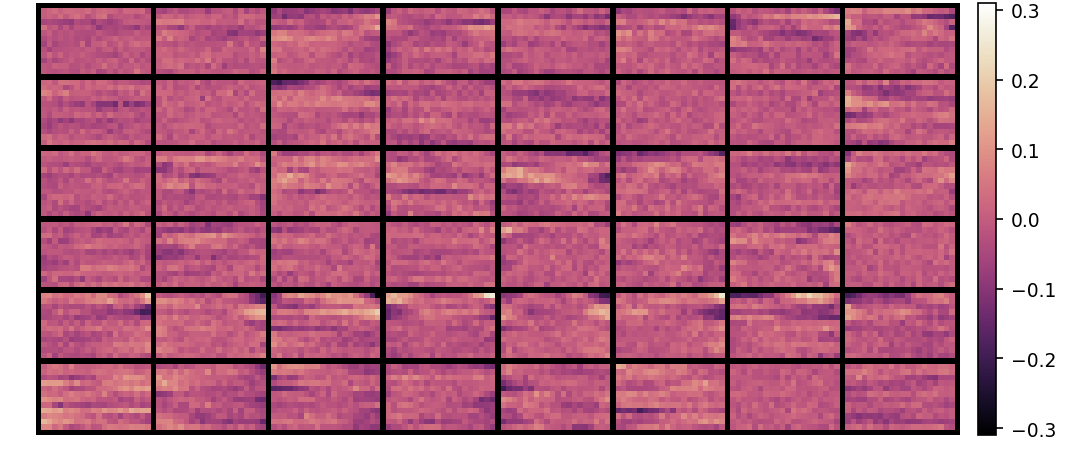
\includegraphics[width=0.45\textwidth]{./4_nn/figs/nn_adv_label_weights_d-1000.png}}
  \caption{Concatenated label weights of the filters in the first convolutional layer from the Discriminator model with different amounts of epochs.}
  \label{fig:nn_adv_label_weights_d}
\end{figure}
\FloatBarrier
\noindent
\begin{figure}[!ht]
  \centering
  \subfigure[G with 100 epochs]{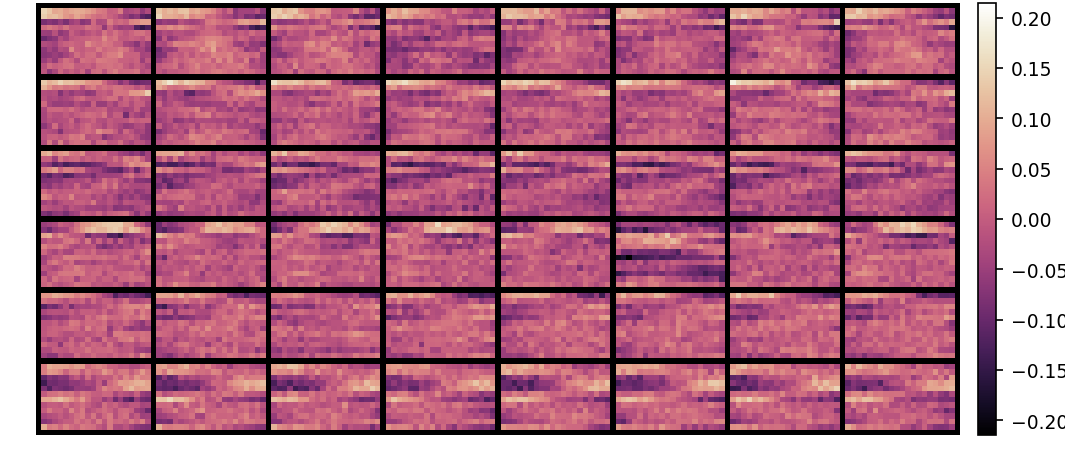
\includegraphics[width=0.45\textwidth]{./4_nn/figs/nn_adv_label_weights_g-100.png}}
  \subfigure[G with 1000 epochs]{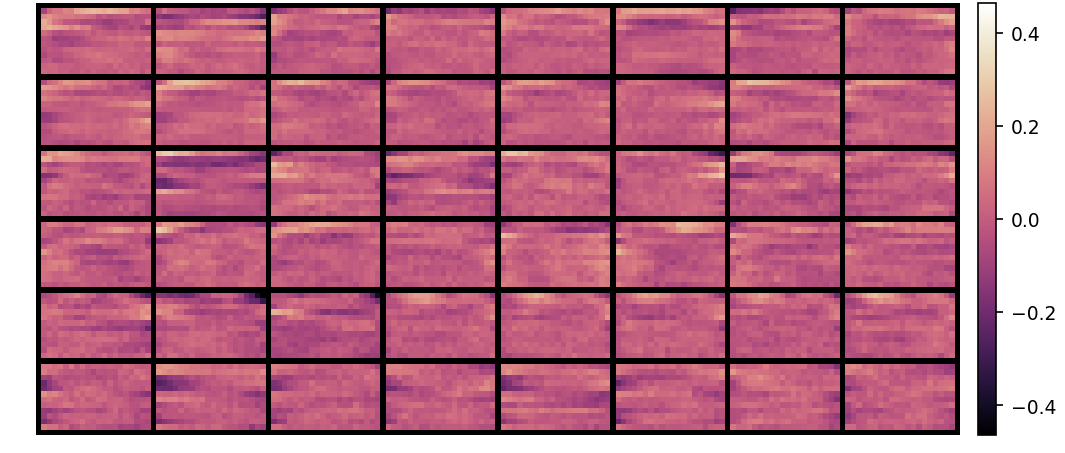
\includegraphics[width=0.45\textwidth]{./4_nn/figs/nn_adv_label_weights_g-1000.png}}
  \caption{Concatenated label weights of the filters in the first convolutional layer from the Generator model with different amounts of epochs.}
  \label{fig:nn_adv_label_weights_g}
\end{figure}
\FloatBarrier
\noindent
The amount of training epochs is important because it determines how much the models learn during their adversarial training.
With 100 training epochs, the Generator already creates similar convolutional filters for each label train instance because it does not need to be that accurate in creating different looking fakes.
However the Discriminator gets better as well and the need of generating different looking fakes motivates G to match up.
With 1000 epochs the Generator generates many different fakes, as already shown in \rfig{nn_adv_fakes_label} and the filters take on different structures. 
Note that a second convolutional layer for the \texttt{adv-d-jim} and \texttt{adv-g-jim} exist as well, the corresponding weights are shown only for the 100 epoch examples in \rfig{nn_adv_label_weights_conv1}.
\begin{figure}[!ht]
  \centering
  \subfigure[D with 100 epochs]{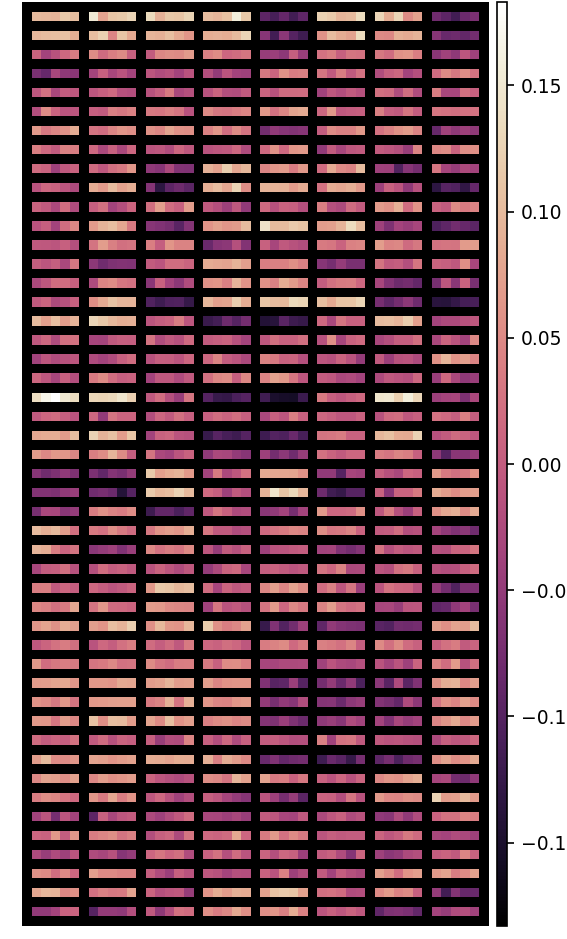
\includegraphics[width=0.25\textwidth]{./4_nn/figs/nn_adv_label_weights_conv1_d-100.png}}
  \qquad \qquad
  \subfigure[G with 100 epochs]{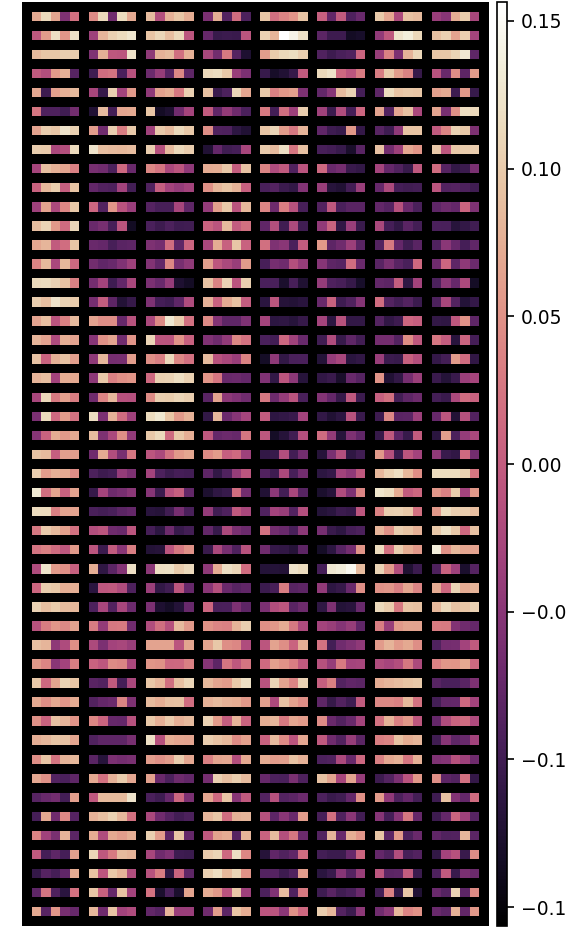
\includegraphics[width=0.25\textwidth]{./4_nn/figs/nn_adv_label_weights_conv1_g-100.png}}
  \caption{Concatenated label weights of the filters in the second convolutional layer from the Discriminator and Generator model trained with 100 epochs.}
  \label{fig:nn_adv_label_weights_conv1}
\end{figure}
\FloatBarrier
\noindent
Each row of the second convolutional layer corresponds to a single feature map produced by the first convolutional layer and therefore 8 rows correspond to one adversarial label training instance.